\begin{frame}{6. Diagram Alir Metodologi (1/2)}
    \centering
    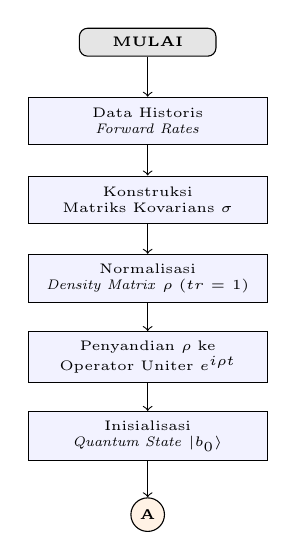
\begin{tikzpicture}[
        node distance=1.0cm,
        every node/.style={fill=white, font=\tiny, align=center},
        block/.style={rectangle, draw, text width=2.8cm, minimum height=0.6cm, fill=blue!5},
        terminal/.style={rectangle, draw, rounded corners=3pt, text width=1.5cm, fill=gray!20, font=\tiny\bfseries},
        connector/.style={circle, draw, fill=orange!10, inner sep=2pt, font=\tiny\bfseries}
    ]
        % Terminals & Pre-processing
        \node (mulai) [terminal] {MULAI};
        \node (start) [block, below of=mulai] {Data Historis \\ \textit{Forward Rates}};
        \node (matriks) [block, below of=start] {Konstruksi \\ Matriks Kovarians $\sigma$};
        \node (norm) [block, below of=matriks] {Normalisasi \\ \textit{Density Matrix} $\rho$ ($\text{tr}=1$)};
        \node (uniter) [block, below of=norm] {Penyandian $\rho$ ke \\ Operator Uniter $e^{i\rho t}$};
        \node (init) [block, below of=uniter] {Inisialisasi \\ \textit{Quantum State} $|b_0\rangle$};
        
        % Terminal Connector A
        \node (connA) [connector, below of=init] {A};

        % Connections
        \draw [->] (mulai) -- (start);
        \draw [->] (start) -- (matriks);
        \draw [->] (matriks) -- (norm);
        \draw [->] (norm) -- (uniter);
        \draw [->] (uniter) -- (init);
        \draw [->] (init) -- (connA);
    \end{tikzpicture}
\end{frame}

\begin{frame}{6. Diagram Alir Metodologi (2/2)}
    \centering
    \begin{tikzpicture}[
        node distance=1.0cm,
        every node/.style={fill=white, font=\tiny, align=center},
        block/.style={rectangle, draw, text width=2.8cm, minimum height=0.6cm, fill=blue!5},
        decision/.style={diamond, draw, aspect=2, text width=1.5cm, fill=yellow!10},
        io/.style={trapezium, trapezium left angle=70, trapezium right angle=110, draw, fill=green!5, text width=2.5cm},
        terminal/.style={rectangle, draw, rounded corners=3pt, text width=1.5cm, fill=gray!20, font=\tiny\bfseries},
        subgraphI/.style={draw, dashed, inner sep=0.3cm, fill=red!5, fill opacity=0.1},
        subgraphII/.style={draw, dashed, inner sep=0.3cm, fill=cyan!5, fill opacity=0.1},
        connector/.style={circle, draw, fill=orange!10, inner sep=2pt, font=\tiny\bfseries}
    ]
        % Entry Connector A
        \node (connA) [connector] {A};
        
        % Tahap I: Iterative Eigenvector Estimation
        \node (evolusi) [block, below of=connA, node distance=1.2cm] {Evolusi Uniter \\ \& QFT};
        \node (proyeksi) [block, below of=evolusi] {Proyeksi pada \\ Estimasi Biner $|y^{(n)}\rangle$};
        \node (stabil) [decision, below of=proyeksi, node distance=1.6cm] {Stabil?};
        \node (isolasi) [block, below of=stabil, node distance=1.5cm] {Ekstraksi Vektor Eigen \\ $|u_{max}\rangle$};

        % Tahap II: Eigenvalue Refinement
        \node (fase) [block, right of=isolasi, node distance=3.8cm] {Rotasi Basis ($x, y, r$) \\ \& Fase Relatif};
        \node (refine) [block, above of=fase, node distance=1.4cm] {\textit{Refinement} \\ Eigenvalue (QPE)};
        \node (mitigasi) [block, above of=refine, node distance=1.4cm] {Mitigasi Galat \\ (Richardson/Readout)};
        
        % Output & Terminal
        \node (result) [io, above of=mitigasi, node distance=1.4cm] {Output: Komponen \\ Utama Model HJM};
        \node (selesai) [terminal, above of=result, node distance=1.2cm] {SELESAI};

        % Connections
        \draw [->] (connA) -- (evolusi);
        \draw [->] (evolusi) -- (proyeksi);
        \draw [->] (proyeksi) -- (stabil);
        \draw [->] (stabil) -- node[anchor=west] {Ya} (isolasi);
        \draw [->] (stabil.west) -- ++(-0.8,0) |- node[anchor=east, pos=0.25] {Belum (\textit{Feedback})} (evolusi.west);
        \draw [->] (isolasi) -- (fase);
        \draw [->] (fase) -- (refine);
        \draw [->] (refine) -- (mitigasi);
        \draw [->] (mitigasi) -- (result);
        \draw [->] (result) -- (selesai);

        % Subgraph Boxes
        \begin{pgfonlayer}{background}
            \node [subgraphI, fit=(evolusi) (proyeksi) (stabil), label={[shift={(0,-0.4)}]above:\textbf{Tahap I: Estimasi Eigenvector Iteratif}}] {};
            \node [subgraphII, fit=(fase) (refine) (mitigasi), label={[shift={(0,-0.4)}]above:\textbf{Tahap II: Refinement Eigenvalue}}] {};
        \end{pgfonlayer}
    \end{tikzpicture}
\end{frame}
